\documentclass[article]{rqPenVignette}%{jss}

%% -- LaTeX packages and custom commands ---------------------------------------

%% recommended packages
\usepackage{thumbpdf,lmodern,amsfonts,amsmath,mathtools}

%% another package (only for this demo article)
\usepackage{framed}

%% new custom commands
\newcommand{\class}[1]{`\code{#1}'}
\newcommand{\fct}[1]{\code{#1()}}

%% REMEMBER WHEN IN DOUBT RUN THE TEX FILE FIRST AND THEN TRY THE SWEAVE FILE

\newcommand{\va}{{\bf a}}
\newcommand{\vb}{{\bf b}}
\newcommand{\vc}{{\bf c}}
\newcommand{\vd}{{\bf d}}
\newcommand{\ve}{{\bf e}}
\newcommand{\vf}{{\bf f}}
\newcommand{\vh}{{\bf h}}
\newcommand{\vl}{{\bf l}}
\newcommand{\vr}{{\bf r}}
\newcommand{\vW}{{\bf W}}
\newcommand{\vS}{{\bf S}}
\newcommand{\vE}{{\bf E}}
\newcommand{\vG}{{\bf G}}
\newcommand{\vF}{{\bf F}}
\newcommand{\vK}{{\bf K}}
\newcommand{\vm}{{\bf m}}
\newcommand{\vp}{{\bf p}}
\newcommand{\vt}{{\bf t}}
\newcommand{\vs}{{\bf s}}
\newcommand{\vu}{{\bf u}}
\newcommand{\vv}{{\bf v}}
\newcommand{\vw}{{\bf w}}
\newcommand{\vx}{{\bf x}}
\newcommand{\vy}{{\bf y}}
\newcommand{\vz}{{\bf z}}
\newcommand{\vA}{{\it A}}
\newcommand{\vB}{{\it B}}
\newcommand{\vC}{{\it C}}
\newcommand{\vH}{{\it H}}
\newcommand{\vI}{{\it I}}
\newcommand{\vJ}{{\it J}}
\newcommand{\vL}{{\it L}}
\newcommand{\vM}{{\it M}}
\newcommand{\vN}{{\it N}}
\newcommand{\vP}{{\it P}}
\newcommand{\vQ}{{\it Q}}
\newcommand{\vq}{{\it q}}
\newcommand{\vR}{{\it R}}
\newcommand{\vT}{{\it T}}
\newcommand{\vU}{{\it U}}
\newcommand{\vV}{{\it V}}
\newcommand{\vX}{{\it X}}
\newcommand{\vY}{{\it Y}}
\newcommand{\vZ}{{\it Z}}
\newcommand{\vD}{{\it D}}
\newcommand{\Fs}{\mathcal{F}}
\newcommand{\ra}{\rightarrow}
\newcommand{\vgamma}{\mbox{\boldmath $\gamma$}}
\newcommand{\vbeta}{\mbox{\boldmath $\beta$}}
\newcommand{\vepsilon}{\mbox{\boldmath $\epsilon$}}
\newcommand{\vxi}{\mbox{\boldmath $\xi$}}
\newcommand{\vpi}{\mbox{\boldmath $\pi$}}
\newcommand{\vtheta}{\mbox{\boldmath $\theta$}}
\newcommand{\valpha}{\mbox{\boldmath $\alpha$}}
\newcommand{\vkappa}{\mbox{\boldmath $\kappa$}}
\newcommand{\Real}{\mathbb{R}}


%% For Sweave-based articles about R packages:
%% need no \usepackage{Sweave}



%% -- Article metainformation (author, title, ...) -----------------------------

%% - \author{} with primary affiliation
%% - \Plainauthor{} without affiliations
%% - Separate authors by \And or \AND (in \author) or by comma (in \Plainauthor).
%% - \AND starts a new line, \And does not.
\author{Ben Sherwood\\University of Kansas
   \And Shaobo Li\\University of Kansas 
   \And Adam Maidman \\ Airbnb}
\Plainauthor{Ben Sherwood, Shaobo Li, Adam Maidman}

%% - \title{} in title case
%% - \Plaintitle{} without LaTeX markup (if any)
%% - \Shorttitle{} with LaTeX markup (if any), used as running title
\title{rqPen: An \proglang{R} package for penalized quantile regression}
\Plaintitle{An R package for penalized quantile regression}
\Shorttitle{rqPen: Penalized quantile regression}

%% - \Abstract{} almost as usual
\Abstract{
  Quantile regression directly models a conditional quantile of interest. A wide variety of 
  penalties have been introduced to improve regression estimation and many all provide 
  simultaneous estimation and model selection. The \proglang{R} package rqPen provides penalized quantile 
  regression for lasso, elastic net, adaptive lasso, SCAD and MCP penalties, along with extensions to group penalties.
  The backbone of the package is the elastic net and group lasso methods, which are of interest in their own right and can be used 
  to approximate the nonconvex penalties. The traditional approach to solving penalized quantile regression problems is to frame it as a linear programming, similar to 
  what is done with unpenalized quantile regression. For large data sets this approach can be computationally burdensome.   The package \pkg{rqPen} provides these traditional linear programming solutions, along with coordinate descent algorithms and algorithms based on approximating the quantile loss with a Huber-type approximation. 
}

%% - \Keywords{} with LaTeX markup, at least one required
%% - \Plainkeywords{} without LaTeX markup (if necessary)
%% - Should be comma-separated and in sentence case.
\Keywords{quantile regression, penalized regression, model selection}
\Plainkeywords{quantile regression, penalized regression, model selection}

%% - \Address{} of at least one author
%% - May contain multiple affiliations for each author
%%   (in extra lines, separated by \emph{and}\\).
%% - May contain multiple authors for the same affiliation
%%   (in the same first line, separated by comma).
\Address{
  Ben Sherwood\\
  School of Business \\ 
  University of Kansas \\
  1654 Naismith Drive\\
  Lawrence, KS, USA 66045 \\ 
  E-mail: \email{ben.sherwood@ku.edu}\\
  URL: \url{https://business.ku.edu/people/ben-sherwood}
}

% \VignetteIndexEntry{rqPen Vignette}

\begin{document}



%% -- Introduction -------------------------------------------------------------

%% - In principle "as usual".
%% - But should typically have some discussion of both _software_ and _methods_.
%% - Use \proglang{}, \pkg{}, and \code{} markup throughout the manuscript.
%% - If such markup is in (sub)section titles, a plain text version has to be
%%   added as well.
%% - All software mentioned should be properly \cite-d.
%% - All abbreviations should be introduced.
%% - Unless the expansions of abbreviations are proper names (like "Journal
%%   of Statistical Software" above) they should be in sentence case (like
%%   "generalized linear models" below).

\section{Introduction} \label{sec:intro}


\cite{origQR} proposed quantile regression as robust alternative to mean regression that 
directly models a conditional quantile of interest without the need for assumptions about the 
distribution or variance of the error term. Since the seminal paper of \citep{lasso}, introducing the lasso penalty, investigating the 
combination of different penalties and loss functions has been an active area of interest. Penalties provided in \pkg{rqPen} are lasso, 
elastic net \citep{zou05}, SCAD \citep{fanLi}, MCP \citep{mcp}, adaptive lasso \citep{adaptiveLasso}, group lasso \citep{yuan2007} and other group extensions of the previously stated penalties \citep{grSCAD, groupReview, penBiLevel}, with the exception of elastic net for which a group generalization has not been implemented. Extending the theoretical results of penalized estimators to the quantile regression setting has been an active area of research. Examples include deriving the rate of convergence for lasso \citep{qr_lasso} and group lasso \citep{qr_group_lasso} and deriving oracle properties for non-convex penalties such as SCAD and MCP \citep{lan_scad}. Discussed in these papers is how minimizing the penalized objective functions for quantile regression can be framed as linear programming problems or, in the case of group lasso, second order cone programming problems. The linear programming formulation is particularly familiar to researchers in quantile regression because this is the most common approach for solving quantile regression problems, including in the \pkg{quantreg} package \citep{crq1,crq2}. While a second order cone programming problem can be solved using convex optimization software, including the R package \pkg{Rmosek} \citep{JSSv060i05}.

The ability to analyze large data sets is one of the major appeals of penalized regression methods. However, linear programming and second order cone programming becomes computationally burdensome for large data sets. Further complicating matters, is the quantile loss function is non-differentiable, while popular algorithms for penalized objective functions rely on a differentiable loss function, for instance \cite{friedman2009glmnet} (elastic net), \cite{scadAlg} (non-convex penalties), \cite{brehenyglasso} (group non-convex penalties),  and \cite{Yang2015} (group lasso). \cite{huber_cd} proposed using a Huber-type approximation of quantile loss and coordinate descent algorithm for solving elastic net penalized quantile regression which is implemented in the \proglang{R} package \pkg{hqreg}. \cite{qr_cd} proposed a coordinate descent algorithm (QICD) for nonconvex penalties that relies on an initial estimator being provided, implemented in \pkg{qicd}. Other approaches, albeit without active \proglang{R} packages, for penalized quantile regression include using ADMM algorithms \citep{admm_nan_qr,lan_admm, admm_hui}. % and a coordinate descent algorithm (QICD) for nonconvex penalties \citep{qr_cd}. %IN ADDITION CITE OUR OWN WORK FOR GROUP LASSO AND R PACKAGE.    

The package \pkg{rqPen} provides implementation of the Huber based approximation, linear programming and QICD. It allows users to fit quantile regression models with all of the penalty functions discussed in the first paragraph. It also provides tools for using cross validation or information criterion for parameter selection. In addition, it provides plots for how cross validation results and coefficient estimation change with $\lambda$, the main sparsity tuning parameter. The package allows for estimation of multiple quantiles and provides plots for how coefficient values change with the quantile being modeled, $\tau$. The packages \pkg{quantreg} and \pkg{hqreg} are other alternative for penalized quantile regression in \proglang{R}. The package \pkg{rqPen} provides access to the same penalties these packages provide, plus additional penalties. For instance, neither of these packages include group penalties. In addition, \pkg{rqPen} provides more tools that are directly catered to penalized regression. Such as the previously mentioned trace plots and using information criterion for parameter selection.   While \pkg{hrqglaso} provides penalized group lasso, it does not provide any of the other group penalties, nor does it allow for simultaneous estimation of multiple quantiles. On the other hand that package and \pkg{hqreg} are also setup to allow for robust mean regression using the Huber loss function, something \pkg{rqPen} is not setup to do. 



%% -- Manuscript ---------------------------------------------------------------

%% - In principle "as usual" again.
%% - When using equations (e.g., {equation}, {eqnarray}, {align}, etc.
%%   avoid empty lines before and after the equation (which would signal a new
%%   paragraph.
%% - When describing longer chunks of code that are _not_ meant for execution
%%   (e.g., a function synopsis or list of arguments), the environment {Code}
%%   is recommended. Alternatively, a plain {verbatim} can also be used.
%%   (For executed code see the next section.)

\section{Penalized estimation of quantile regrssion} \label{sec:models}
Consider observations $\{y_i,\vx_i\}_{i=1}^n$, where $\vx_i \in \Real^p$, and the model
\begin{equation}
\label{qrModel}
y_i = \vx_i^\top \vbeta^{\tau}_0 + \epsilon_i,
\end{equation}
where $P(\epsilon_i < 0 | \vx_i)=\tau$. Define $\rho_\tau(u) = u[\tau-I(u<0)]$ and \citet{origQR} proposed estimating \eqref{qrModel} by minimizing
\begin{equation}
\label{qr}
\sum_{i=1}^n \rho_\tau(y_i-\vx_i^\top\vbeta),
\end{equation}
which is available in the package \pkg{quantreg}. The package \pkg{rqPen} provides functions for estimating $\vbeta^\tau_0$ by minimizing 
\begin{equation*}
\frac{1}{n} \sum_{i=1}^n \rho_\tau(y_i - \vx_i^\top\vbeta) + \lambda P_a(\vbeta).
\end{equation*}

The penalty function $P_a(\vbeta)$ can take on the form of a group or individual penalty. 

\subsection{Individual Penalties}

The package \pkg{rqPen} supports four different forms of individual penalties. The SCAD, $p^s_{\lambda,a}()$, and MCP, $p^m_{\lambda,a}()$ penalty functions are 
\begin{eqnarray*}
p^s_{\lambda,a}(|x|) &=& \lambda|x|I(0 \leq |x| < \lambda) + \frac{a\lambda|x|-(x^2+\lambda^2)/2}{a-1}I(\lambda \leq |x| \leq a\lambda) + \frac{(a+1)\lambda^2}{2}I(|x|>a\lambda),  \\
p^m_{\lambda,a}(|x|) &=& \lambda(|x|-\frac{x^2}{2a\lambda})I(0 \leq |x| < a\lambda) + \frac{a\lambda^2}{2}I(|x|\geq a\lambda),  
\end{eqnarray*}
where $a>2$ for the SCAD penalty function and $a>1$ for MCP. 

The following are the four different penalty functions, plus two important special cases. 

\begin{enumerate}
\item Elastic net: $P_a(\vbeta) = \lambda \sum_{j=1}^p w_j \left[ \alpha |\beta_j| +  (1-\alpha) \beta_j^2 \right]$, where $a \in [0,1]$. 
\begin{enumerate}
\item LASSO: special case with $a=1$.
\item Ridge: special case with $a=0$. 
\end{enumerate}
\item Adaptive LASSO: $P_a(\vbeta) = \lambda \sum w_j |\tilde{\beta}_j|^{-a} |\beta_j|$, where $a>0$. 
\item SCAD: $P_a(\vbeta) = \sum_{j=1}^p p^s_{w_j\lambda,a}(|\beta_j|)$, where $a>2$.
\item MCP: $P_a(\vbeta) = \sum_{j=1}^p p^m_{w_j\lambda,a}(|\beta_j|)$, where $a>1$. 
\end{enumerate}

The weights, $w_j$, allow for different weights for each predictor and most be non-negative. If $w_j=0$ then that variable will be unpenalized and thus is guaranteed to be included in the model. In \pkg{rqPen} these weights are refereed to as \emph{penalty.factors} or \emph{group.penalty.factors}. The value $\tilde{\beta}_j$ is the coefficient of the Ridge estimator with the same value of $\lambda$. The LASSO estimator provides the backbone for the algorithm of the three non-elastic net penalties. As $\rho_\tau(x)+\rho_\tau(-x) = |x|$, the LASSO estimator minimizes,
\begin{equation}
\label{lasso}
\frac{1}{n} \sum_{i=1}^n \rho_\tau(y_i - \vx_i^\top\vbeta) +  \sum_{j=1}^p \rho_\tau(\lambda w_j\beta_j)+\rho_\tau(-\lambda w_j\beta_j).
\end{equation}
For $i \in \{1,\ldots,n\}$ define $\tilde{y}_i = y_i$ and $\tilde{\vx}_i = \vx_i$. Let $\ve_j \in \Real^{p+1}$ represent a unit vector with a value of one in the jth position and zero in all other entries. For $i \in \{n+1,\ldots,n+2p\}$, $\tilde{\vx}_i = -n\lambda w_j \ve_j$ or $\tilde{\vx}_i = n\lambda w_j \ve_j$, where each definition is used once for each value of $j \in \{1,\ldots,p\}$. While, $\tilde{y}_i = 0$ for $i \in \{n+1,\ldots,n+2p\}$. Then minimizing \eqref{lasso} is equivalent to minimizing 
\begin{equation}
\label{lassoAlt}
\frac{1}{n} \sum_{i=1}^{n+2p} \rho_\tau(\tilde{y}_i-\tilde{\vx}_i^\top\vbeta),
\end{equation}
which, with the exception of the scaling constant of $\frac{1}{n}$, has the same form as \eqref{qr}. This approach of creating the augmented 2p samples and then using standard quantile regression is implemented in \pkg{rqPen} where the problem is solved using the \emph{rq()} function from \pkg{quantreg}. Note this approach is different than using \emph{method=``lasso''} within \pkg{quantreg}. Below is code for fitting a lasso penalized estimator to the \emph{barro} data set from \pkg{rqPen} using the ``br'' and ``fn'' algorithms from quantreg. Where the ``br'' implementation is described in \citet{crq1} and \citet{crq2}, while implementation of ``fn'' is decribed in \citet{portnoy1997}. Our experience is that ``br'' performs better and is more likely to provide a sparse solution.

\begin{Schunk}
\begin{Sinput}
R> library(rqPen)
R> #quantreg is required for rqPen, but call directly here
R> #because we need the barro data set
R> library(quantreg)
R> data(barro)
R> y <- barro$y.net
R> x <- as.matrix(barro[,-1])
R> qbr <- rq.pen(x,y,alg="br")
R> qfn <- rq.pen(x,y,alg="fn")
\end{Sinput}
\end{Schunk}

For large values of $n$ and $p$ the linear programming algorithms become computationally burdensome. To decrease computational complexity, \citet{huber_cd} proposed approximating the quantile loss function with a Huber-like function and proposed a new coordinate descent algorithm that requires a differentiable loss function. Define the Huber loss function proposed by \citet{huber1964} as
\begin{eqnarray*}
	h_\gamma(t) = \begin{dcases}
		\frac{t^2}{2\gamma}, & \mbox{ if } |t| \leq \gamma,\\
		|t|-\frac{\gamma}{2}, & \mbox{ if } |t| > \gamma.
	\end{dcases}
\end{eqnarray*}
Note $\rho_\tau(u) = u[\tau-I(u<0)]=\frac{1}{2}(|u|+(2\tau-1)u)$ and for sufficiently small $\gamma$, $|u| \approx h_\gamma(u)$. We define the Huber-approximated quantile loss as
\begin{equation}
\label{huber_quantile}
h_{\gamma}^{\tau}(u) = h_\gamma(u) + (2\tau-1)u,
\end{equation}
and for small $\gamma$, $\rho_\tau(u) \approx \frac{1}{2}h_{\gamma}^{\tau}(u)$. The package \pkg{hqreg} implements the approach of \citet{huber_cd} and the function \emph{hqreg()}, with \emph{method=``quantile''} solves the problem of
\begin{equation}
\label{huberLasso}
\frac{1}{2n} \sum_{i=1}^n h_{\gamma}^{\tau}(y_i - \vx_i^\top\vbeta) +  \lambda \sum_{j=1}^p w_j|\beta_j|.
\end{equation}

This implementation can be used in \pkg{rqPen} by the following code.   

\begin{Schunk}
\begin{Sinput}
R> qhuber <- rq.pen(x,y,alg="huber")
\end{Sinput}
\end{Schunk}

Setting \emph{alg="huber"} calls \emph{hqreg::hqreg()}, and thus \pkg{hqreg} is another required package for \pkg{rqPen}. The Huber approximation is the default and will be used if the algorithm is not specified.  The LASSO penalty provides the backbone for the three non-elastic net algorithms. For the adaptive LASSO the connection is straight forward, as it is a special case of a LASSO problem with different weights for each coefficients. The initial estimators necessary for the weights are determined by a ridge estimator with the same value of $\lambda$. The SCAD and MCP functions are approximated by a local linear approximation (LLA) as proposed by \citet{lla}. Let $p_{w_j\lambda,a}(|\beta_j|)$ represent a generic penalty function and $p'_{w_j\lambda,a}(|\beta_j|)$ be the derivative with respect to $\beta_j$. In addition let $\bar{\beta}_j$ be the LASSO estimator for the same value of $\lambda$ and weights. The LLA approach uses the following approximation, 
\begin{equation}
\label{lla}
\sum_{j=1}^p p_{w_j\lambda,a}(|\beta_j|) \approx \sum_{j=1}^p p'_{w_j\lambda,a}(|\bar{\beta}_j|)|\beta_j|.
\end{equation}
Again, the problem becomes a special case of a LASSO estimator with specific weights for each predictor. Thus all the non-elastic net penalties can be solved using the linear programming or the Huber approximation algorithms. \citet{qr_cd} proposed a coordinate descent algorithm for penalized objective functions with quantile loss and a non-convex penalty (QICD). This approach has been implemented for the SCAD and MCP functions. That proposed algorithm requires a good initial estimator and \pkg{rqPen} uses a lasso estimator. For this reason the algorithm was not implemented for the LASSO penalty. For larger values of p and n this algorithm is faster than linear programming approaches. The Huber based algorithm will be faster than QICD, but the trade-off there is using an approximation for the quantile loss function. 

%ADAM, DO YOU WANT TO FILL IN SOME QICD DETAILS HERE? 

The elastic net penalty of 
\begin{equation}
\label{enet}
\frac{1}{n} \sum_{i=1}^n \rho_\tau(y_i - \vx_i^\top\vbeta) + \lambda \sum_{j=1}^p w_j \left[ a|\beta_j|+(1-a)\beta_j^2\right],
\end{equation}
cannot be framed as a linear programming problem because of the ridge penalty. Thus for $a \neq 1$, the \pkg{rqPen} implementation of elastic net uses the Huber approximation approach provided in \pkg{hqreg}. While \pkg{hqreg} provides a computational backbone, \pkg{rqPen} provides additional functions that will be described later. In addition the next section includes group penalties, that are not implemented in \pkg{hqreg}. For some group penalties \pkg{hqreg} will still provide a computational backbone, but for other penalties it will not be used. 


\subsection{Group Penalties}

Group penalties are useful when there is a group structure to the predictors. Common examples of this are non-binary categorical variables or polynomial transformations of single predictor. This section assumes the $p$ predictors are partitioned into $G$ groups and $\vbeta_g$ represents the coefficients associated with the $g$th group of predictors. Group penalized quantile regression estimators minimize
\begin{equation}
\label{groupForm}
\frac{1}{n} \sum_{i=1}^n \rho_\tau(y_i - \vx_i^\top\vbeta) + \sum_{g=1}^G p_{w_g\lambda,a}(||\vbeta_g||_q).
\end{equation}

Group penalties are implemented for four penalty functions: (1) LASSO; (2) Adaptive LASSO; (3) SCAD; and (4) MCP. Currently, there is no implementation of a group elastic net or ridge penalty. For the latter there does not exist a group version of the ridge penalty. For the former, that would be a convex combination of a group lasso penalty and ridge. Implementing this would require generalizing the group lasso penalty algorithm and has not been done, yet. All four functions use the same form presented in the previous subsection, but the scalar $\beta_j$ is replaced with the scalar $||\vbeta_g||_q$. The choice q is limited to $q \in \{1,2\}$. If $q=2$ then group variable selection will be all-or-nothing, that is all variables within a group will be selected or none of them will be. The choice of $q=1$, allows for bi-level variable selection, that is it is possible to have zero and non-zero estimates for coefficients within a group. Consider the case of the LASSO penalty for $q=1$ \eqref{groupForm} is 
\begin{equation}
\label{l1glasso}
\frac{1}{n} \sum_{i=1}^n \rho_\tau(y_i - \vx_i^\top\vbeta) + \sum_{g=1}^G w_g||\vbeta_g||_1,
\end{equation}
while for $q=2$ it is 
\begin{equation}
\label{l2glasso}
\frac{1}{n} \sum_{i=1}^n \rho_\tau(y_i - \vx_i^\top\vbeta) + \sum_{g=1}^G w_g||\vbeta_g||_2.
\end{equation}
Note that \eqref{l1glasso} is a special case of the individual LASSO penalty where the weights within each group are the same, while \eqref{l2glasso} is the standard group lasso penalty introduced by \citet{yuan2007}. The estimator that minimizes \eqref{l1glasso} is not guaranteed to have variable selection agreement within a group, where this is guaranteed for the estimator that minimizes \eqref{l2glasso}. Due to \eqref{l1glasso} being a special case of the individual lasso estimator it is not implemented as a group penalty, but for all other penalty functions users can choose between $q=1$ or $q=2$. These other three penalties are partially motivated by a desire to have the oracle property. However, for $q=1$ it has been shown that the oracle property only holds at the group level and not at the individual level, although these results do not explore the non-differentiable quantile loss function or the adaptive lasso penalty \citep{mestatp}. For an excellent review of group penalties, including a discussion of the use of $q=1$ the reader is referred to \citet{groupReview}. \citet{penBiLevel} provides a more detailed exploration of group penalties with $q=1$. 

Choosing $q=1$ for quantile regression estimators has the additional benefit of being solved using linear programming, the most commonly used approach for quantile regression problems. As mentioned previously the group LASSO estimator becomes a special case of the individual LASSO estimator, and this is also true for the adaptive LASSO penalty. For the SCAD and MCP penalties the same LLA will be used. Again let $\bar{\vbeta}_g$ be an initial group LASSO estimator and the penalized objective function is approximated by 
\begin{equation}
\label{groupFormlla}
\frac{1}{n} \sum_{i=1}^n \rho_\tau(y_i - \vx_i^\top\vbeta) + \sum_{g=1}^G p'_{w_g\lambda,a}(||\bar{\vbeta}_g||_q)||\vbeta_g||_q.
\end{equation}

For the case of $q=1$ this becomes an individual LASSO problem and the algorithms discussed in the previous section apply, though with some minor differences that will be discussed in the following section. While for $q=2$ this becomes a special case of the group LASSO problem. These group LASSO problems are not linear programming problems, but second-order cone programming problems. Therefore they can be solved by existing convex optimization software such as \pkg{Rmosek} \citep{JSSv060i05}. However, there are some barriers to a user in using \pkg{Rmosek}. A user needs to correctly define all the variables of the convex optimization problem and they need to have a copy of Mosek installed on their computer. In addition, similar to linear programming problems, second-order cone programming problems can be computationally burdensome for large values of $n$ or $p$. For $q=2$, the Huber approximation described in the previous subsection is used. However, \pkg{hqreg} cannot be used to solve this problem because the approach of \citet{huber_cd} is not for a group penalty. Instead the algorithm of \citet{Yang2015} is implemented. %, see OURPAPER for specific details regarding the application of this algorithm to the quantile regression setting. This approach is available in the package \pkg{hrqglas}, which is maintained by two of the authors, and is used as the computational backbone for the $L2$ group penalties. 

%SHAOBO, WOULD BE VERY HELPFUL IF YOU ADDED SOME DETAILS ABOUT THE GROUP PENALTY 

\subsection{Estimation of Multiple Quantiles}

The previous two subsections considers only one quantile, but, similar to \pkg{quantreg}, \pkg{rqPen} accommodates estimation of multiple quantiles. Consider B quantiles and let $\tau_b$ be the $b$th quantile of interest. Let $\vbeta^{\tau_b}$ be the regression coefficients for the $b$th quantile.  For individual penalties the estimator minimizes,
\begin{equation}
\label{multtau}
\frac{1}{n} \sum_{b=1}^B\sum_{i=1}^n \rho_\tau\left(y_i - \vx_i^\top\vbeta^{\tau_b}\right) + \sum_{b=1}^B\sum_{j=1}^p p_{w_jd_b\lambda,a}(|\beta^{\tau_b}_j|).
\end{equation}
While for group penalties it is
\begin{equation}
\label{multtaug}
\frac{1}{n} \sum_{b=1}^B \sum_{i=1}^n \rho_\tau\left(y_i - \vx_i^\top\vbeta^{\tau_b}\right) + \sum_{b=1}^B \sum_{g=1}^G p_{w_gd_b\lambda,a}(||\vbeta_g||_q).
\end{equation}
The main difference is the introduction of quantile specific weights for the penalty terms. \citet{qr_lasso} provide one example of specific weights for each quantiles and use $d_b = \sqrt{\tau_b(1-\tau_b)}/n$. Dividing by $n$ is simply a difference in the scale of $\lambda$, but the $\sqrt{\tau_b(1-\tau_b)}$ term provides a quantile dependent weight. The optimization of \eqref{multtau} and \eqref{multtaug} consist of $B$ different optimization problems that have been discussed in Sections 2.1 and 2.2. 

\subsection{Tuning parameter selection}
There are two tuning parameters, $\lambda$ and $a$, that need to be set. The value of $a$ defaults to commonly used values for each penalty: (1) elastic-net (a=1); (2) adaptive LASSO (a=1); (3) SCAD (a=3.7); and (4) MCP (a=3). Users can also specify their own value of $a$ or a sequence of potential values of $a$ to be considered. Users can specify their own sequence for values of $\lambda$, otherwise a sequence will be automatically generated. Define $H_\gamma^\tau(\vbeta) = \frac{1}{2n} \sum_{i=1}^n h_\gamma^\tau(y_i - \vx_i^\top\vbeta)$. Define $\tilde{a}=a$ if the elastic net penalty is used and zero otherwise. The default value for individual penalties is $\lambda_{\max} = \max_{j,b} 1.05\left|\frac{\partial}{\partial \beta_j} H_\gamma^{\tau_b}(\mathbf{0}_{p+1})\right|(w_jd_b\tilde{a})^{-1}$ and for the group penalties is $\lambda_{\max} = \max_{g,b} 1.05\left|\left| \frac{\partial}{\partial \vbeta_g} H_\gamma^{\tau_b}(\mathbf{0}_{p+1})\right|\right|_q (w_gd_b)^{-1}$. Without the 1.05 multiplier, these values of $\lambda_{\max}$ provide a totally sparse solution for LASSO and group LASSO under the KKT conditions of the Huber approximation. However, not all algorithms use the Huber approximation and the 1.05 multiplier is used to make it more likely that $\lambda_{\max}$ will provide a totally sparse solution for any estimator. If any predictors or groups are unpenalized at a given quantile then they are excluded from these calculations.

Both cross-validation and information criterion are provided as tools for selecting the optimal pair of $(\lambda,a)$. For a given quantile $\tau$ and pair of tuning parameters $(\lambda,a)$ with estimator $\hat{\vbeta}^\tau_{\lambda,a}$ with $k^\tau_{\lambda,a}$ non-zero coefficients, including the intercept, define the quantile information criterion (QIC) as 
\begin{equation}
\label{qic}
QIC(\tau,\lambda,a) = \log\left[ \sum_{i=1}^n \rho_\tau(y_i-\vx_i^\top \hat{\vbeta}^\tau_{\lambda,a}) \right] + mk^\tau_{\lambda,a}, 
\end{equation}
where the value of $m$ depends on the criterion being used. In \pkg{rqPen} the user can select between AIC ($m=2$), BIC [$m=\log(n)$] and a version of the large $p$ BIC proposed by \citet{qrbic} [$m=\log(n)\log(p)$]. Using the barro data set used previously,  below is code for modeling the $.25$ quantile using elastic net and results for using both AIC and BIC to select the pair of $(\lambda,a)$.

\begin{Schunk}
\begin{Sinput}
R> rqe <- rq.pen(x,y,tau=.25,penalty="ENet",a=seq(0,1,.1),alg="huber")
R> aicm <- qic.select(rqe, method="AIC")
R> #BIC is the default method
R> bicm <- qic.select(rqe)
R> #following returns the coefficients of the selected model
R> coefficients(bicm)
\end{Sinput}
\begin{Soutput}
          tau=0.25
 [1,] -0.040226686
 [2,] -0.023893370
 [3,]  0.006519105
 [4,]  0.003225629
 [5,]  0.000000000
 [6,]  0.000000000
 [7,]  0.059605464
 [8,] -0.001406846
 [9,] -0.215479802
[10,]  0.090625321
[11,] -0.140849188
[12,] -0.025810735
[13,] -0.029461310
[14,]  0.079574971
\end{Soutput}
\begin{Sinput}
R> #provides information about the selected model
R> bicm$modelsInfo
\end{Sinput}
\begin{Soutput}
    tau modelIndex a   minQIC lambdaIndex      lambda
1: 0.25         11 1 6.388936         100 0.001960444
\end{Soutput}
\begin{Sinput}
R> #provides IC values for all possible models
R> bicm$ic[1:5,1:5]
\end{Sinput}
\begin{Soutput}
   tau0.25a0 tau0.25a0.1 tau0.25a0.2 tau0.25a0.3 tau0.25a0.4
L1  22.27022    10.87212    9.657005    8.883748    8.441887
L2  22.26040    10.87212    9.657005    8.883748    8.441887
L3  22.25236    10.87212    9.657005    8.883748    8.441887
L4  22.24375    10.87212    9.657005    8.883748    8.441887
L5  22.23495    10.87212    9.657005    8.883748    8.441887
\end{Soutput}
\end{Schunk}


For the case of multiple, $B$, quantiles being modeled, \pkg{rqPen} offers two different approaches for selecting the tuning parameters. One approach is to select $B$ pairs of $(\lambda,a)$ that minimize the $B$ different versions of \eqref{qic}. Define $B$ weights of $(w_1,\ldots,w_B)$. The other approach is to select a single pair of $(\lambda,a)$ that minimizes,
\begin{equation}
\sum_{b=1}^B w_b QIC(\tau_b,\lambda,a).
\end{equation}
The weights offer flexibility to a user who wants to provide more weight to a specific quantile. The default value for all the weights is one thus giving equal weight to each quantile. Below is code implementing both approaches. Note in this case the two approaches provide identical results, that is optimizing $\lambda$ uniquely for each $\tau$ provides the same $\lambda$ for all values of $\tau$. However, this is not guranteed to happen. 

\begin{Schunk}
\begin{Sinput}
R> #lasso model for 9 quantiles
R> tvals <- seq(.1,.9,.1)
R> rqmt <- rq.pen(x,y,tau=tvals)
R> #default is to find the optimal value of 
R> # lambda for each quantile separately
R> rqmt_st <- qic.select(rqmt)
R> # alternative option is to find one value of 
R> # lambda best for all tau. Below code
R> # also provides different weights for the models
R> rqmt_g <- qic.select(rqmt,septau = FALSE,weights=sqrt(tvals*(1-tvals)))
R> # first one will have different values of lambda for each quantile
R> # second approach will provide the same value for lambda for all quantiles
R> rqmt_st$modelsInfo
\end{Sinput}
\begin{Soutput}
   tau modelIndex a    minQIC lambdaIndex      lambda
1: 0.1          1 1 11.202792         100 0.001995633
2: 0.2          2 1 13.345651         100 0.001995633
3: 0.3          3 1 14.039835         100 0.001995633
4: 0.4          4 1 14.254535         100 0.001995633
5: 0.5          5 1 14.190048         100 0.001995633
6: 0.6          6 1 14.935143         100 0.001995633
7: 0.7          7 1 14.262631         100 0.001995633
8: 0.8          8 1 12.989257         100 0.001995633
9: 0.9          9 1  9.611465         100 0.001995633
\end{Soutput}
\begin{Sinput}
R> rqmt_g$modelsInfo
\end{Sinput}
\begin{Soutput}
         modelIndex a tau    minQIC lambdaIndex      lambda
tau0.1a1          1 1 0.1 11.202792         100 0.001995633
tau0.2a1          2 1 0.2 13.345651         100 0.001995633
tau0.3a1          3 1 0.3 14.039835         100 0.001995633
tau0.4a1          4 1 0.4 14.254535         100 0.001995633
tau0.5a1          5 1 0.5 14.190048         100 0.001995633
tau0.6a1          6 1 0.6 14.935143         100 0.001995633
tau0.7a1          7 1 0.7 14.262631         100 0.001995633
tau0.8a1          8 1 0.8 12.989257         100 0.001995633
tau0.9a1          9 1 0.9  9.611465         100 0.001995633
\end{Soutput}
\begin{Sinput}
R> #below command gets coefficients for the selected model optimized for each quantile
R> coefficients(rqmt_st)
\end{Sinput}
\begin{Soutput}
           tau=0.1      tau=0.2      tau=0.3       tau=0.4
 [1,]  0.046024550 -0.025349510 -0.007628702 -0.0509099459
 [2,] -0.026284237 -0.024599504 -0.024662593 -0.0269258058
 [3,]  0.012328949  0.008081397  0.006480841  0.0064768621
 [4,]  0.002104772  0.005166707  0.002814568  0.0000000000
 [5,] -0.024627664 -0.025607695  0.007792513 -0.0006238768
 [6,]  0.009512346  0.008764757  0.000000000  0.0040800327
 [7,]  0.042289169  0.058181214  0.053186347  0.0687972724
 [8,] -0.001056290 -0.001910715 -0.001721006 -0.0009412972
 [9,] -0.362402003 -0.307690904 -0.094324088 -0.0775372750
[10,]  0.088922202  0.079340696  0.086755769  0.0830892163
[11,] -0.205922592 -0.167878400 -0.144565626 -0.1236879324
[12,] -0.024300727 -0.024496546 -0.029762941 -0.0285998471
[13,] -0.026985871 -0.031168065 -0.031536259 -0.0321213531
[14,]  0.108965090  0.113462718  0.090556363  0.1079694258
           tau=0.5      tau=0.6      tau=0.7      tau=0.8
 [1,] -0.030427445 -0.027667070 -0.036468569 -0.059369918
 [2,] -0.025921439 -0.027154054 -0.027049752 -0.029731119
 [3,]  0.010717433  0.012767446  0.020075468  0.020387034
 [4,]  0.000000000  0.000000000 -0.005597457 -0.007651144
 [5,]  0.000000000  0.004500418  0.000000000 -0.017975998
 [6,]  0.005652769  0.012718075  0.008847529  0.012003063
 [7,]  0.061545816  0.064704621  0.066847390  0.077466640
 [8,] -0.002032809 -0.003109405 -0.003002686 -0.002238763
 [9,] -0.053542693 -0.118189204 -0.097732410  0.099465610
[10,]  0.079649154  0.078695159  0.069455746  0.054449904
[11,] -0.096936333 -0.101068296 -0.098374165 -0.079401138
[12,] -0.026219888 -0.029832149 -0.027298837 -0.029925264
[13,] -0.029603500 -0.023199084 -0.017604570 -0.006516214
[14,]  0.150465797  0.193290866  0.203671322  0.217579350
           tau=0.9
 [1,] -0.031105032
 [2,] -0.032783674
 [3,]  0.019155652
 [4,] -0.005962290
 [5,] -0.001556920
 [6,]  0.004491901
 [7,]  0.078839376
 [8,] -0.002483301
 [9,] -0.047988988
[10,]  0.062508461
[11,] -0.090451700
[12,] -0.032571747
[13,]  0.003103054
[14,]  0.227296281
\end{Soutput}
\begin{Sinput}
R> #code is the same for a group penalty
R> # This is not a great use of a group penalty and only for
R> # example
R> g <- c(rep(1,4),rep(2,3),rep(3,3),rep(4,3))
R> rqgroup <- rq.group.pen(x,y,groups=g,tau=seq(.1,.9,.1))
R> rqgroup_ic <- qic.select(rqgroup)
\end{Sinput}
\end{Schunk}

Cross-validation is the other implemented approach for choosing the optimal pair of $(\lambda,a)$. Consider the case of $K$ folds, let $n_k$ be the number of observations in the $k$th fold, $y_i^k$ and $\vx_i^k$ be the $i$th response and predictor vector for the $k$th fold and $\hat{\vbeta}^{\tau_b}_{-k,\lambda,a}$ be the fit for the $b$th quantile excluding the $k$th fold for given values of $\lambda$ and $a$. By default, even if Huber approximations are used, cross-validation is done with respect to quantile loss. However, this can be changed by setting \emph{cvFunc}, for instance \emph{cvFunc=abs} will use absolute value loss regardless of the quantile being modeled. For simplicity of presentation the following assumes quantile loss is used. The average quantile loss at a given fold is 
\begin{equation}
\label{cv1}
C_k^\tau(\lambda,a) = \frac{1}{n_k} \sum_{i=1}^{n_k} \rho_\tau(y_i^k-{\vx_i^k}^\top\hat{\vbeta}^{\tau}_{-k,\lambda,a}).
\end{equation}
The cross-validation functions return two summaries of the cross validation for selecting $(\lambda,a)$. The return value \emph{btr} provides a table of the values of $a$ and $\lambda$ that minimize 
\begin{equation}
\label{cv2}
C^\tau(\lambda,a) = \frac{1}{K} \sum_{k=1}^K C_k^\tau(\lambda,a).
\end{equation}
In addition it provides the $\lambda$ that provides the sparsest solution that is within one standard error of the value that minimizes \eqref{cv2}, with $a$ fixed. The standard error is calculated as 
\begin{equation}
\sqrt{\frac{1}{K-1} \sum_{k=1}^K \left[C_k^\tau(\lambda,a)-C^\tau(\lambda,a) \right]^2},
\end{equation}
The average summary can be replaced by changing the parameter \emph{cvSummary}, for instance \emph{cvSummary=median} would use the median values of $C_k^\tau(\lambda,a)$. The return value \emph{gtr} provides results for the value of $\lambda$ and $a$ that minimize
\begin{equation}
\label{cv3}
C(\lambda,a) = \sum_{b=1}^B w_b C^{\tau_b}(\lambda,a).
\end{equation}
Thus, again, providing the option to optimize the tuning parameters jointly or separately across quantiles. %The results also include results for the one standard error approach. %Let $(a_{\mbox{opt}},\lambda_{\mbox{opt}})$ represent the optimal pair, which may change depending on the quantile or if \eqref{cv2} or \eqref{cv3} is minimized. 
%For minimizing \eqref{cv2} the standard error for a given value of $(\lambda,a)$ the  
%\begin{equation}
%\sqrt{\frac{1}{K-1} \sum_{k=1}^K \left[C_k^\tau(\lambda,a)-C^\tau(\lambda,a) \right]^2},
%\end{equation}
%while for minimizing \eqref{cv3} the standard error is 
%\begin{equation}
%\sqrt{\frac{1}{K-1}\sum_{k=1}^K \left[\sum_{b=1}^B w_b C_k^\tau(\lambda,a) -C(\lambda,a) \right]^2}.
%\end{equation}
%NOT 100\% SURE THIS IS THE RIGHT APPROACH AND HAVE NOT IMPLEMENTED YET. wILL IMPLEMENT ONCE WE AGREE/DISCUSS. 
%The one standard error rule than finds the sparsest solution, by increasing $\lambda$, where the value of \eqref{cv2} or \eqref{cv3} are within one standard error of the optimal value, assuming the optimal $a$ is fixed. 

By setting \emph{groupError=FALSE} each cross-validation error is weighted equally and \eqref{cv2} and \eqref{cv3} are replaced by 
\begin{equation}
\label{gf1}
\sum_{k=1}^K n_k C_k^\tau(\lambda,a),
\end{equation}
and
\begin{equation}
\label{gf2}
\sum_{b=1}^B w_b \sum_{k=1}^K n_k C_k^\tau(\lambda,a),
\end{equation}
respectively. 
%With \emph{groupError=FALSE} the standard error calculations remain the same and using the one standard error rule with \emph{groupError=FALSE} may be sub-optimal. 



\subsection{Additional notes on Huber approximation}

For Huber approximation an appropriate value of $\gamma$ is needed. If the value is too large then the estimator will have a large amount of bias, but if the value is too small the algorithms will become unstable. The values of $\gamma$ are updated for each value of $\lambda$. Let $\vr^k$ be the vector of residuals corresponding to the estimator using the $k$th value of $\lambda$, $\lambda^k$, and $Q_{.1}(|\vr^k|)$ be the 10th percentile of the absolute values of these residuals. For the individual penalties we use the approach outlined by \citet{huber_cd}, with differences only coming from later changes that were made in \pkg{hqreg},
\begin{eqnarray*}
\gamma^k &=& I(|1-\tau|< .05)\max\left\{.0001,\min\left[\gamma^{k-1},Q_{.01}(|\vr^k|)\right]\right\} \\
&& + I(|1-\tau|>=.05)\max\left\{.001,\min\left[\gamma^{k-1},Q_{.1}(|\vr^k|)\right]\right\}.
\end{eqnarray*}

For the group penalties%, as presented in CITE-OUR-PAPER,
\begin{equation*}
\gamma^k = \min\left\{4, \max\left[.001, Q_{.1}(|\vr^k|) \right] \right\}.
\end{equation*}

Generally speaking, $\gamma$ needs to be small, but not too small. For larger values of $\gamma$ the approximation becomes closer to a least squares or expectile loss function \citep{expectile}. As expectile regression is not the same as quantile regression and least squares is only the same if the errors are symmetric, this can result in biased estimators. For values of $\gamma$ that are too small the algorithms become unstable as the differentiable loss function becomes for practical purposes non-differentiable. Our experience has been that the automated methods work well. The cautious user can specify a fixed value of  $\gamma$ for \code{rq.group.pen}, but \pkg{hqreg} does not offer this flexibility and thus only the automatic values of $\gamma$ are used for \code{rq.pen}. 

One reason the linear and second-order cone programming problems are computationally slow for larger values of $p$ is they optimize with respect to all the potential covariates. \citet{tibshirani2012strong} proposed a strong rule for discarding predictors that can greatly decrease the computational complexity of penalized optimization. The strong rule assumes a differentiable loss function and thus is only implemented for the Huber approximations. In addition the Huber approximation approaches use warm starts across a path of potential $\lambda$ values. It starts with the largest potential value of $\lambda$ then uses that solution as the initial value for the next largest potential value of $\lambda$. This iterative process is continued until all solutions have been found. The linear programming approaches rely on \emph{quantreg::rq()} that does not have an option for initial values. Thus warm starts are not implemented for those approaches. For the individual penalties, the calculations of the strong rule are down in the package \pkg{hqreg}, and details can be found in \citet{huber_cd}. A similar approach has been used for the group penalties. %For group penalties, SHAOBO CAN YOU FILL IN DETAILS HERE? 


\section{Description of functions}
Below are the main functions of \pkg{rqPen} and an S3 method that is unique to \pkg{rqPen}, \code{bytau.plot},
\begin{itemize}
\item \fct{rq.pen} provides estimates of a quantile regression model, for potentially multiple quantiles, using an individual penalty of either elastic-net, adaptive LASSO, SCAD or MCP. If not specified, will automatically generate a sequence of $\lambda$ values. Returns an \class{rq.pen.seq} S3 object that works \code{bytau.plot}, \code{coef}, \code{plot}, \code{predict}, and \code{print} methods. 
\item \fct{rq.group.pen} is a group penalty version of \fct{rq.pen}. Users have access to group versions of LASSO, adaptive LASSO, SCAD and MCP. The LASSO penalty is restricted to the L2-norm, but for other penalties users can choose between the L1 or L2 norm. It also returns an an \class{rq.pen.seq} S3 object and can be used with the same methods listed above. 
\item \fct{rq.pen.cv} automates K-folds cross-validation for selection of the tuning parameters $\lambda$ and $a$. A sequence of $\lambda$ will be automatically generated. However, for $a$ a sequence needs to be supplied, otherwise a single default value will be used. If multiple quantiles are modeled then finds the optimal pair of $(\lambda,a)$ for each quantile and the optimal pair across all quantiles.  Returns an \class{rq.pen.seq.cv} S3 object that works with \code{bytau.plot}, \code{coef}, \code{plot}, \code{predict}, and \code{print} methods.  
\item \fct{rq.group.pen.cv} is the group version of \fct{rq.pen.cv}. It does everything listed above, but for group penalties. It also returns an \class{rq.pen.seq.cv} object. 
\item \fct{QIC.select} takes a \class{rq.pen.seq} object and provides the optimal values of $(\lambda,a)$ using information criterion explained in the previous section. It returns a \class{qic.select} S3 object that works with \code{coef}, \code{predict} and \code{print} methods. 
\item \fct{bytau.plot} plots coefficients estimates for each predictor as a function of $\tau$. 
\end{itemize}

Below are descriptions of \code{rq.pen} and \code{rq.pen.cv} and their arguments. These functions are very similar to \code{rq.group.pen} and \code{rq.group.pen.cv}. In addition, some of the arguments in \code{rq.pen.cv} are simliar to those of \code{qic.select}. The next section includes examples of using all of these functions. 

Below is the \code{rq.pen} function, followed by its arguments. 
\\
\code{rq.pen(x, y, tau = 0.5, lambda = NULL,
        penalty = c("LASSO", "Ridge", "ENet", "aLASSO", "SCAD", "MCP"),
        a = NULL, nlambda = 100, eps = ifelse(nrow(x) < ncol(x), 0.05, 0.01),
        penalty.factor = rep(1, ncol(x)), alg = ifelse(sum(dim(x)) < 200, "br", "huber"),
        scalex = TRUE, 
        tau.penalty.factor = rep(1, length(tau)), coef.cutoff = 1e-08,
        max.iter = 10000, converge.eps = 1e-07, lambda.discard = TRUE,...)}
\\
\begin{itemize}
\item[\code{x}] Matrix of predictor values. 
\item[\code{y}] Vector of response. 
\item[\code{tau}] Vector of quantiles being modeled, default is to only model the median.
\item[\code{lambda}] Vector of lambda values. If not specified then a sequence will be automatically generated based on the data and rules described in previous section. 
\item[\code{penalty}] Penalty used, choices are LASSO, Ridge, elastic-net ("ENet"), adaptive LASSO ("aLASSO"), SCAD or MCP. 
\item[\code{a}] Additional tuning parameter, not used for lasso or ridge penalties. However, will be set to the elastic net values of 1 and 0 respectively. Defaults are ENet(0), aLASSO(1), SCAD(3.7) and MCP(3).
\item[\code{nlambda}] The number of lambdas generated. This is ignored if lambda is set manually. 
\item[\code{eps}] Multiplied by $\lambda_{\max}$ to define $\lambda_{\min}$ when the sequence of lambda values is generated automatically. If $n<p$ it defaults to .05, otherwise it defaults to .01. 
\item[\code{penalty.factor}] Weights for the penalty for each predictor, the value $w_j$ from \eqref{multtau}. Default is to provide a value of one for each predictor, thus weighting them all equally. 
\item[\code{alg}] The algorithm used. Default is ``huber'', the algorithm described in \citet{huber_cd}. Linear programming solutions can be obtained using ``br'' or ``fn'' corresponding to the same algorithms available in \code{quantreg::rq}.  Our experience has shown "br" to perform better than ``fn'' because it tends to provide a sparse solution, but it can be slow. The ``QICD'' algorithm is available for MCP or SCAD. For elastic net, Ridge or adaptive LASSO the choice must be "huber".
\item[\code{scalex}] If set to TRUE, the default, the x matrix will be centered and scaled to have mean zero and standard deviation of one. Coefficients are returned on the original scale of the data. 
\item[\code{tau.penalty.factor}] Weights for the coefficients of each quantile, the value $d_b$ from \eqref{multtau}. Default provides equal weight, of one, for each quantile 
\item[\code{coef.cutoff}] Some of the linear programming algorithms will provide very small, but not sparse solutions. Estimates below this number will be set to zero. This is ignored if a non-linear programming algorithm is used.
\item[\code{max.iter}] Maximum number of iterations of non-linear programming algorithms.
\item[\code{converge.eps}] Convergence threshold for non-linear programming algorithms.
\item[\code{lambda.discard}] Algorithm may stop for small values of lambda if the coefficient estimates are not changing drastically. One example of this is it is possible for the LLA weights of the non-convex functions, see \eqref{lla},  to all become zero and smaller values of lambda are extremely likely to produce the same zero weights.
\end{itemize}

Below is the \code{rq.pen.cv} followed by its arguments. \\
\code{rq.pen.cv(x, y, tau = 0.5, lambda = NULL,
  penalty = c("LASSO", "Ridge", "ENet", "aLASSO", "SCAD", "MCP"),
  a = NULL, cvFunc = NULL, nfolds = 10, foldid = NULL,
  nlambda = 100, groupError = TRUE, cvSummary = mean,
  tauWeights = rep(1, length(tau)), printProgress = FALSE, ...)}
\\
\begin{itemize}
\item[\code{x}] Matrix of predictor values. 
\item[\code{y}] Vector of response. 
\item[\code{tau}] Vector of quantiles being modeled, default is to only model the median.
\item[\code{lambda}] Vector of lambda values. If not specified then a sequence will be automatically generated based on the data and rules described in previous section. 
\item[\code{penalty}] Penalty used, choices are LASSO, Ridge, elastic-net ("ENet"), adaptive LASSO ("aLASSO"), SCAD or MCP. 
\item[\code{a}] Additional tuning parameter, not used for lasso or ridge penalties. However, will be set to the elastic net values of 1 and 0 respectively. Defaults are ENet(0), aLASSO(1), SCAD(3.7) and MCP(3).
\item[\code{cvFunc}] Loss function for cross-validation. Defaults to quantile loss, but user can specify their own function.
\item[\code{folds}] Number of folds, $K$, used for $K$-folds cross validation. 
\item[\code{foldid}] A vector of length $n$ of fold assignments. If this is set, then \code{folds} is ignored. 
\item[\code{nlambda}] The number of lambdas generated. This is ignored if lambda is set manually. 
\item[\code{groupError}] If true then tuning parameters the by tau results, btr, are found to minimize \eqref{}. 
\item[\code{...}] Additional arguments passed to \code{rq.pen}. 
\end{itemize}

% Outline
% 
% 1. rq.pen()
% 2. rq.group.pen()
% 3. rq.pen.cv()
% 4. rq.group.pen.cv()
% 5. QIC.select()
% 
% Mention of downstream applications
% 
% 1. coefficients
% 2. predict
% 3. plot
% 4. bytau.plot

\section{Applications}
This section details fitting using the aforementioned barro data set and the Ames housing data \citep{de2011ames}. %In both examples, multiple values of $\tau$ and $a$ will be considered, but by no means is this necessary. To accommodate the multiple values of $a$, which do not apply to the LASSO or group LASSO penalties, an elastic net penalty will be used for the individual penalties and a group SCAD penalty will be used for the group example. %The examples will demonstrate how to fit the model, select tuning parameters, produce plots and make predictions from the optimal models. 

\subsection{barro}

The barro data set, available in \pkg{quantreg}, contains GPD growth rates and 13 other potential explanatory variables. See \citet{barro} for more details. The following will provide code on fitting an elastic net model with potential 11 potential $a$ values from 0 to 1 and equally spaced out by .1. Similarly, we will model 9 quantiles equally spaced out from .1 to .9. The below code fits models for the 9 different models, automatically generates a sequence of $\lambda$ and considers the 11 potential $a$ values using the Huber approximation algorithm. 
\begin{Schunk}
\begin{Sinput}
R> quants <- seq(.1,.9,.1)
R> r1 <- rq.pen(x,y,a=seq(0,1,.1),tau=quants,penalty="ENet",alg="huber")
R> #Below plots the coefficient values for .1 quantile with a=.1
R> plot(r1,a=.1,tau=.1,logLambda = TRUE)
R> #Below code would provide plots for all possible values of a and tau
R> #plot(r1,logLambda=TRUE)
\end{Sinput}
\end{Schunk}
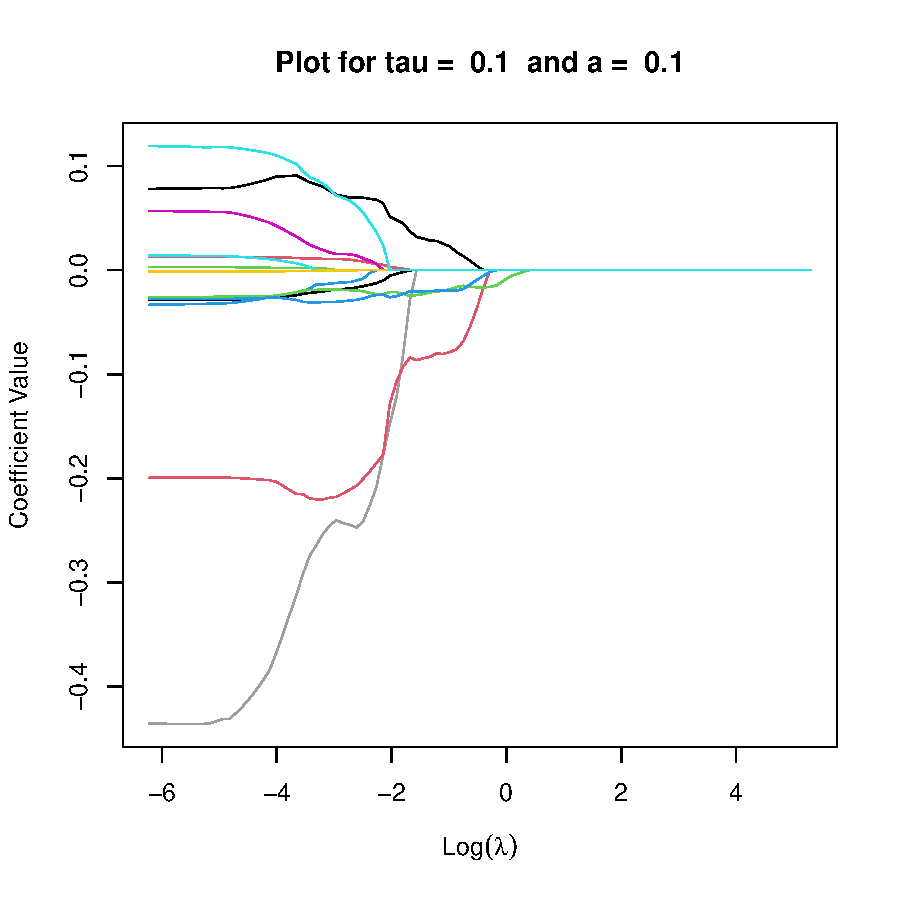
\includegraphics{article-006}


\subsection{Group Penalty Example}
The Ames Housing data contains many factor variables and is available in \pkg{AmesHousing}. Below is an example of cross validation code used to fit a model for the median using the group lasso penalty. The plot demonstrates the cross-validation error as a function of $\lambda$. 
\begin{Schunk}
\begin{Sinput}
R> library(AmesHousing)
R> ames <- make_ames()
R> x_g <- cbind(model.matrix(~ Lot_Shape+Garage_Type+Full_Bath
+                            +Fireplaces+Lot_Config - 1,ames))
R> y_g <- log(ames$Sale_Price)
R> g <-  c(rep(1,4),rep(2,6),3,4,rep(5,4))
R> r2 <- rq.group.pen.cv(x_g,y_g,groups=g)
R> plot(r2)
\end{Sinput}
\end{Schunk}
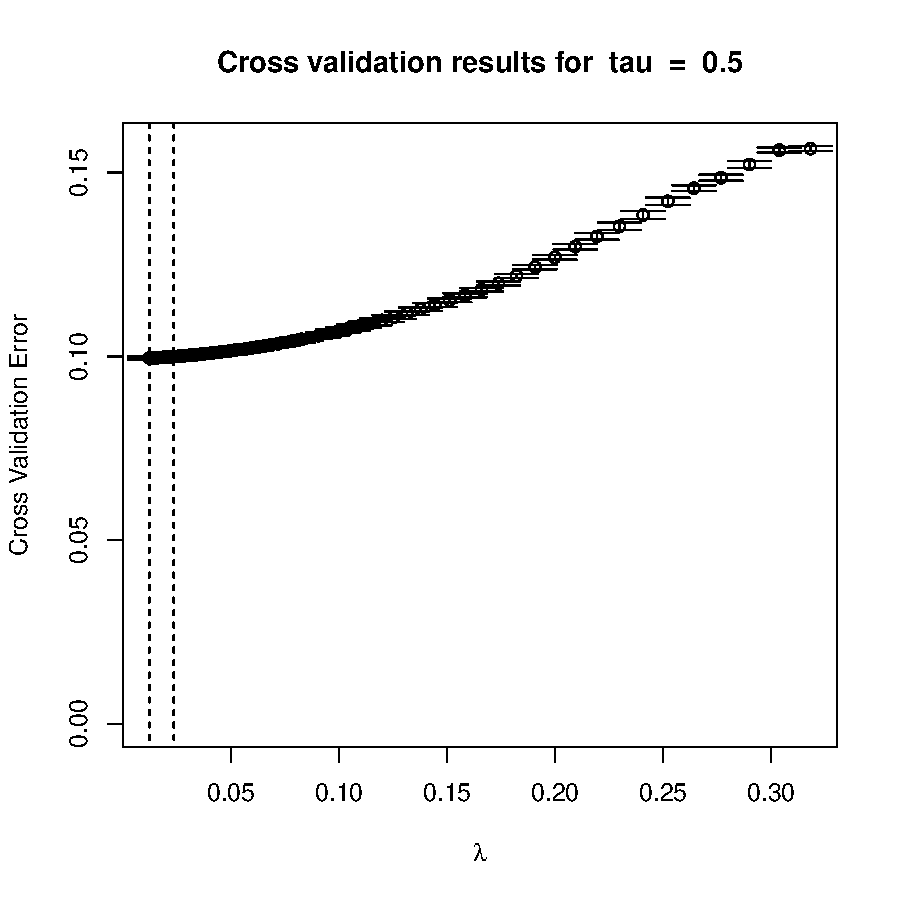
\includegraphics{article-007}

\section{Conclusion}
The \pkg{rqPen} provides tools for penalized estimators of quantile regression models. The package supports elastic-net, adaptive LASSO, SCAD and MCP penalty functions for both individual and group penalties, though for group penalties only the special case of LASSO is available for elastic-net. It provides three different approaches for estimating these models: (1) linear programming; (2) QICD based approaches; and (3) Huber-like approximation of the quantile loss function with coordinate descent algorithms. The package is currently available on CRAN and github, see \url{https://github.com/bssherwood/rqpen} for the most recent updates. 



\bibliography{refs}


%% -- Appendix (if any) --------------------------------------------------------
%% - After the bibliography with page break.
%% - With proper section titles and _not_ just "Appendix".


\end{document}
